\documentclass[UTF8,a4paper,zihao=-4,fontset=windows]{ctexart}

\usepackage[margin=2.55cm]{geometry}
\usepackage{amsmath,amssymb}
\usepackage{booktabs}
\usepackage{tabularx}
\usepackage{longtable}
\usepackage{array}
\usepackage{makecell}
\usepackage{graphicx}
\usepackage{xcolor}
\usepackage{enumitem}
\usepackage{caption}
\usepackage{subcaption}
\usepackage{tikz}
\usepackage{placeins}
\usepackage{xurl}
\usepackage[numbers,sort&compress]{natbib}
\usepackage[colorlinks=true,linkcolor=black,citecolor=black,urlcolor=blue!45!black]{hyperref}
\hypersetup{
  pdftitle={近期 3R 模型综述：前馈式三维重建的表示、时序与输出},
  pdfauthor={},
  pdfsubject={3R and feed-forward 3D reconstruction survey},
  pdfkeywords={3R, feed-forward 3D reconstruction, DUSt3R, pointmap, dynamic scene, long-sequence reconstruction, 3D Gaussian Splatting}
}

\usetikzlibrary{arrows.meta,positioning,fit,calc,shapes.geometric}

\setlength{\parindent}{2em}
\setlength{\parskip}{0.15em}
\linespread{1.16}
\emergencystretch=2em
\raggedbottom

\newcolumntype{Y}{>{\raggedright\arraybackslash}X}
\newcolumntype{C}[1]{>{\centering\arraybackslash}p{#1}}
\captionsetup{font=small,labelfont=bf}

\title{\bfseries 近期 3R 模型综述：\\前馈式三维重建的表示、时序与输出}
\author{}
\date{2026年5月}

\begin{document}

\maketitle

\begin{abstract}
DUSt3R 之后，一批前馈式三维重建模型开始以 pointmap、深度、相机、轨迹和置信度等几何中间量为核心接口，弱化传统 SfM/MVS 对显式匹配和相机初始化的依赖。本文围绕这一变化综述近期 3R 文献：MASt3R 和 MASt3R-SfM 侧重匹配与经典几何接口，Fast3R、MV-DUSt3R+、VGGT、MapAnything 和 Pow3R 处理多视角输入、统一几何预测与外部先验，MonST3R、POMATO、D\textsuperscript{2}USt3R、Easi3R 和 RayMap3R 面向动态场景，CUT3R、Spann3R 及后续流式模型讨论状态、记忆和缓存，Test3R、TTT3R、G-CUT3R 关注测试时修正，Splatt3R、InstantSplat、NoPoSplat 则把重建结果接入 Gaussian 表示。本文不对模型作未验证排行，而是按输入假设、输出表示、机制差异和证据来源进行比较。综述表明，近期 3R 的主要问题已经从单次点图预测扩展到尺度一致性、动态干扰、长序列状态维护、先验冲突和可查看输出的可信度等方面。
\end{abstract}

\noindent\textbf{关键词：} 3R；前馈式三维重建；DUSt3R；点图；视觉几何；动态场景；长序列重建；3D Gaussian Splatting

\section{引言}

传统三维重建通常从显式几何流程展开：先提取局部特征并建立匹配，再估计相机位姿、三角化稀疏点，最后通过多视角立体、深度融合或 bundle adjustment 得到更完整的场景表示。这类流程的优点是变量含义明确，失败原因相对容易追溯；不足是对纹理、视角重叠、相机初始化和全局优化质量都较敏感，在无序图片、手持视频和动态场景中常需要额外的筛选、初始化和后处理。

DUSt3R 将上述流程的一部分中间变量改写为稠密 pointmap 预测：给定图像输入，模型输出每个像素对应的三维点及置信度，再通过对齐或下游过程派生相机、深度、点云和匹配信息\citep{dust3r}。这一表示并不消除尺度和一致性问题，但它提供了一个可被后续方法复用的几何接口。MASt3R、Fast3R、VGGT、CUT3R、MonST3R 等工作大多是在这个接口上分别处理匹配、多视角规模、统一几何输出、长序列状态或动态干扰\citep{mast3r,fast3r,vggt,cut3r,monst3r}。

本文所称 3R，主要指以神经网络前馈预测几何中间量的三维重建方法，讨论范围包括图像对、多视角集合、视频、动态场景、长序列以及可渲染输出。Depth Anything、DINOv2、CoTracker、SAM2 等深度、特征、跟踪和分割模型并非本文主线模型，但它们经常作为先验或辅助信号进入 3R 系统，因而在相关章节一并说明\citep{depth_anything,depth_anything_v2,dinov2,cotracker,sam2}。3DGS 与 4DGS 则作为输出表示和渲染背景处理\citep{gaussian_splatting_3d,gaussian_splatting_4d}。

全文先讨论传统几何流程与 pointmap 表示的关系，再依次梳理基础模型、多视角扩展、动态场景、长序列机制、测试时修正和可渲染输出。最后两节回到复现证据、失败样本和开放问题，目的是区分论文机制、官方实现和应用质量之间的证据层级。

\section{从传统几何流程到点图表示}

前馈式三维重建与传统流程的差别，集中在几何量被预测和校正的顺序上。传统 SfM/MVS 把匹配、位姿、三角化、稠密化与融合分为若干显式阶段；pointmap 路线则把每个像素的三维落点当作中间语言，使深度、对应关系、点云和局部相机关系可以在同一表示下讨论。

这种变化的整体对照见图\,\ref{fig:paradigm}。在 pointmap 接口下，多种几何量被放到同一预测框架中，模型可以在相机先验不完整时处理无序图像、稀疏视角和未知内参输入；匹配也不再局限于二维 descriptor 检索，而可以借助三维几何 grounding 接入 SfM 与全局对齐\citep{mast3r,mast3r_sfm}。同时，时间维度上的一致性变得更难处理。成对 pointmap 的组合并不能自然保证长序列稳定，因此后续视频和流式模型必须重新设计状态更新、记忆管理和缓存策略。

\begin{figure}[t]
\centering
\resizebox{\textwidth}{!}{
\begin{tikzpicture}[
  stage/.style={draw, rounded corners=2pt, minimum width=2.55cm, minimum height=0.9cm, align=center, font=\small},
  trad/.style={stage, fill=gray!5},
  fr/.style={stage, fill=blue!4},
  rowlab/.style={font=\small\bfseries, anchor=east},
  arrow/.style={-{Stealth[length=2mm]}, line width=0.45pt}
]
\node[trad] (t1) at (0,0) {特征提取\\与匹配};
\node[trad, right=0.35cm of t1] (t2) {相机位姿\\估计};
\node[trad, right=0.35cm of t2] (t3) {稀疏三角化};
\node[trad, right=0.35cm of t3] (t4) {稠密 MVS\\或深度融合};
\node[trad, right=0.35cm of t4] (t5) {全局 BA\\与稀疏点云};
\foreach \a/\b in {t1/t2, t2/t3, t3/t4, t4/t5} \draw[arrow] (\a) -- (\b);

\node[fr] (r1) at (0,-2.1) {图像 / 图像对\\或多视角};
\node[fr, right=0.35cm of r1] (r2) {pointmap / 深度\\相机 / 置信度};
\node[fr, right=0.35cm of r2] (r3) {对齐与\\一致性检查};
\node[fr, right=0.35cm of r3] (r4) {点云 / 相机 /\\匹配 / Gaussian};
\foreach \a/\b in {r1/r2, r2/r3, r3/r4} \draw[arrow] (\a) -- (\b);

\node[rowlab] at ($(t1.west)+(-0.25,0)$) {传统 SfM/MVS};
\node[rowlab] at ($(r1.west)+(-0.25,0)$) {3R 前馈};
\end{tikzpicture}}
\caption{传统 SfM/MVS 与 3R 前馈预测流程对照。3R 将多种几何中间量前馈预测出来，再通过对齐与一致性检查接入下游表示。}
\label{fig:paradigm}
\end{figure}

本文将 DUSt3R 之后的文献分为六个相互关联的方向：匹配与 SfM 接口、多视角与统一几何、动态与 4D 场景、长序列状态与记忆、测试时修正，以及可视化/资产输出。图 \ref{fig:lineage} 给出综述性谱系，图 \ref{fig:timeline} 给出这些工作的时间分布。

\begin{figure}[t]
\centering
\resizebox{\textwidth}{!}{
\begin{tikzpicture}[
  node distance=0.8cm and 1.1cm,
  root/.style={draw, rounded corners=2pt, fill=gray!8, minimum width=2.5cm, minimum height=0.75cm, align=center, font=\small\bfseries},
  branch/.style={draw, rounded corners=2pt, fill=blue!4, minimum width=3.3cm, minimum height=0.68cm, align=center, font=\small},
  item/.style={draw, rounded corners=2pt, fill=white, minimum width=3.3cm, minimum height=0.62cm, align=center, font=\footnotesize},
  arrow/.style={-{Stealth[length=2mm]}, line width=0.45pt, draw=black!65}
]
\node[root] (dust) {DUSt3R\\点图与置信度};

\node[branch, right=1.4cm of dust, yshift=2.7cm] (match) {匹配与 SfM 接口};
\node[item, right=0.7cm of match] (matchi) {MASt3R；MASt3R-SfM};

\node[branch, right=1.4cm of dust, yshift=1.55cm] (many) {多视角与统一几何};
\node[item, right=0.7cm of many] (manyi) {Fast3R；MV-DUSt3R+；VGGT；MapAnything；Pow3R};

\node[branch, right=1.4cm of dust, yshift=0.4cm] (dyn) {动态与 4D 场景};
\node[item, right=0.7cm of dyn] (dyni) {MonST3R；POMATO；D\textsuperscript{2}USt3R；Easi3R；RayMap3R};

\node[branch, right=1.4cm of dust, yshift=-0.75cm] (stream) {长序列状态与记忆};
\node[item, right=0.7cm of stream] (streami) {CUT3R；Spann3R；Point3R；STream3R\\LONG3R；LoGeR；Mem3R；OVGGT 等};

\node[branch, right=1.4cm of dust, yshift=-1.9cm] (test) {测试时验证与更新};
\node[item, right=0.7cm of test] (testi) {Test3R；TTT3R；G-CUT3R；SfM consistency};

\node[branch, right=1.4cm of dust, yshift=-3.05cm] (out) {可视化与资产输出};
\node[item, right=0.7cm of out] (outi) {Splatt3R；InstantSplat；NoPoSplat；3DGS/4DGS};

\foreach \x in {match,many,dyn,stream,test,out} \draw[arrow] (dust.east) -- (\x.west);
\foreach \a/\b in {match/matchi,many/manyi,dyn/dyni,stream/streami,test/testi,out/outi} \draw[arrow] (\a.east) -- (\b.west);
\end{tikzpicture}}
\caption{DUSt3R 之后的 3R 模型谱系。该图按问题分支组织代表工作。}
\label{fig:lineage}
\end{figure}
\FloatBarrier

\begin{figure}[t]
\centering
\resizebox{\textwidth}{!}{
\begin{tikzpicture}[
  yearlab/.style={font=\small\bfseries, anchor=south},
  tracklab/.style={font=\small\bfseries, anchor=east, align=right},
  cell/.style={draw, rounded corners=2pt, fill=blue!4, align=center, font=\footnotesize, minimum width=3.2cm, inner sep=3pt},
  track/.style={draw=black!40, dashed, line width=0.4pt}
]

\def\xA{0}
\def\xB{3.6}
\def\xC{7.2}
\def\xD{10.8}

\def\yA{0}
\def\yB{-1.3}
\def\yC{-2.6}
\def\yD{-4.3}
\def\yE{-6.0}

\node[yearlab] at (\xA, 0.85) {2023};
\node[yearlab] at (\xB, 0.85) {2024};
\node[yearlab] at (\xC, 0.85) {2025};
\node[yearlab] at (\xD, 0.85) {2026};

\node[tracklab] at (\xA-1.9, \yA) {基础与匹配};
\node[tracklab] at (\xA-1.9, \yB) {多视角与\\统一几何};
\node[tracklab] at (\xA-1.9, \yC) {动态与 4D};
\node[tracklab] at (\xA-1.9, \yD) {长序列与记忆};
\node[tracklab] at (\xA-1.9, \yE) {测试时与输出};

\foreach \y in {0, -1.3, -2.6, -4.3, -6.0}
  \draw[track] (\xA-1.5, \y) -- (\xD+1.7, \y);

\node[cell] at (\xA, \yA) {DUSt3R};
\node[cell] at (\xB, \yA) {MASt3R\\MASt3R-SfM};
\node[cell] at (\xC, \yA) {MapAnything};

\node[cell] at (\xB, \yB) {MV-DUSt3R+};
\node[cell] at (\xC, \yB) {Fast3R\\VGGT\\Pow3R};

\node[cell] at (\xB, \yC) {MonST3R\\Align3R};
\node[cell] at (\xC, \yC) {POMATO\\D\textsuperscript{2}USt3R\\Easi3R};
\node[cell] at (\xD, \yC) {RayMap3R};

\node[cell] at (\xB, \yD) {Spann3R};
\node[cell] at (\xC, \yD) {CUT3R, Point3R\\STream3R\\LONG3R};
\node[cell] at (\xD, \yD) {LoGeR, Mem3R\\OVGGT, LongStream\\PAS3R, FILT3R};

\node[cell] at (\xB, \yE) {Splatt3R\\InstantSplat\\NoPoSplat};
\node[cell] at (\xC, \yE) {Test3R, TTT3R\\G-CUT3R};

\end{tikzpicture}}
\caption{3R 模型谱系的时间分布。横轴为年份（2023--2026），纵向按主分支组织。同一格内模型顺序无含义，仅列入正文引用的代表工作。}
\label{fig:timeline}
\end{figure}
\FloatBarrier

\section{基础谱系：DUSt3R、MASt3R 与 SfM 接口}

DUSt3R 的影响首先体现在表示层面。它把图像对映射到稠密三维点图，并用置信度描述预测可靠性；多视角输入则通过成对预测与全局对齐组织起来\citep{dust3r}。这一能力与 CroCo 的跨视角补全预训练有关，后者已经使网络能够在视觉层面建立 cross-view 对应，DUSt3R 进一步将这种能力转到稠密 pointmap 预测上\citep{croco}。需要指出的是，pointmap 表示并没有解决所有下游困难。长序列、动态物体、遮挡、尺度漂移和大规模多图仍然需要后续模型分别处理。

MASt3R 将上述几何接口用于图像匹配。它在 DUSt3R 的 pointmap 解码器之外加入 dense local feature head，在像素位置输出 descriptor，并用对比损失约束几何对应像素在 descriptor 空间中的距离\citep{mast3r}。推理时，模型先由互最近邻得到 dense correspondence，再利用 pointmap 作为几何先验进行筛选。这样得到的对应关系同时受局部描述子和全局几何约束，在弱纹理、重复结构或遮挡边界附近通常比直接从 pointmap 取最近邻更稳。MASt3R-SfM 将这一匹配能力接回经典 SfM，用于图像检索、对应估计和无约束场景的全局重建\citep{mast3r_sfm}。这说明 3R 表示并不是要取消传统几何，而是为匹配、检索和 bundle adjustment 提供新的输入条件。

\section{多视角规模化与统一视觉几何}

视角规模是 DUSt3R 类方法扩展时最先遇到的问题之一。若仍以图像对为基本单位，图像数量增加后会带来大量成对组合与对齐开销。Fast3R 因此采用 many-view one-forward-pass 路线，面向上千图像级别的前馈重建\citep{fast3r}。与之相对，MV-DUSt3R+ 关注稀疏视角输入，通过多视角 decoder 和 cross-reference fusion 在少量视角下完成单阶段重建\citep{mvdust3rplus}。两者处理的输入规模不同，但都在重新分配“成对对齐”和“多图汇聚”之间的计算预算。

VGGT 将 camera、depth、pointmap 和 tracks 放在同一视觉几何预测框架下，使 3R 从单一点图预测扩展到多种几何量的联合估计\citep{vggt}。MapAnything 在 metric feed-forward reconstruction 中允许内参、位姿、深度和部分重建等可选条件进入模型\citep{mapanything}；Pow3R 则把 camera 与 scene priors 作为可选模态用于前馈预测\citep{pow3r}。这些工作共同表明，多视角 3R 的难点不只是增加输入图像数量，还在于相机、深度、轨迹、尺度和外部先验之间的约束如何同时成立。

这些模型的实验结果需要连同输入规模、分辨率和硬件设置一起阅读。MV-DUSt3R+ 在 12/20 视角场景中给出秒级重建示例，并在 HM3D、ScanNet、MP3D 等数据上比较 MVS、位姿和 NVS 指标；Fast3R 的系统表报告单张 A100 上 2 到 1500 视角的耗时与显存，强调从成对全局对齐转向一次多视角前馈后的代价变化；VGGT 则在单图、少量图像和数百张图像输入下同时输出相机、深度、点图和轨迹\citep{mvdust3rplus,fast3r,vggt}。图\,\ref{fig:paper-core} 对照 DUSt3R 与 VGGT 的方法图：前者突出 pointmap 作为中间表示，后者强调多种几何量的联合预测。

\begin{figure}[!htbp]
\centering
\begin{subfigure}{0.88\textwidth}
\centering
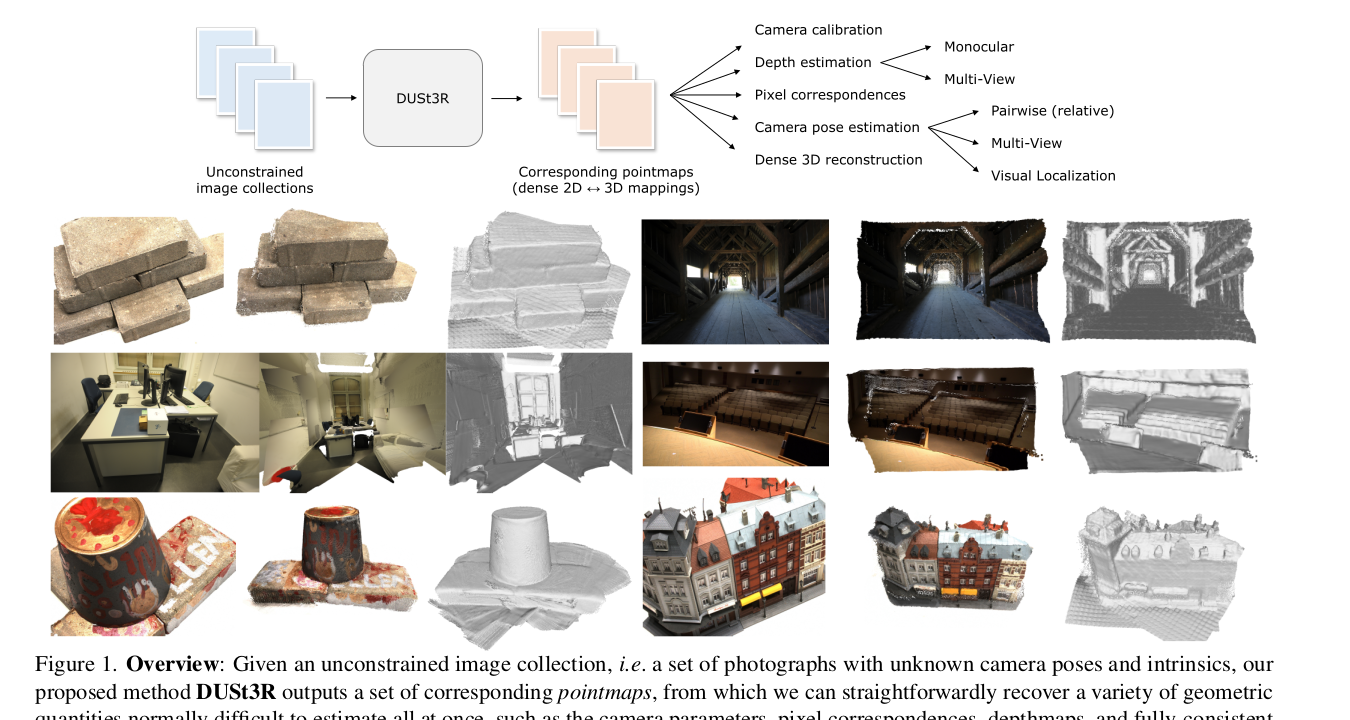
\includegraphics[width=\textwidth]{figures/dust3r_fig1.png}
\caption{DUSt3R}
\label{fig:paper-dust3r}
\end{subfigure}
\vspace{0.5em}
\begin{subfigure}{0.88\textwidth}
\centering
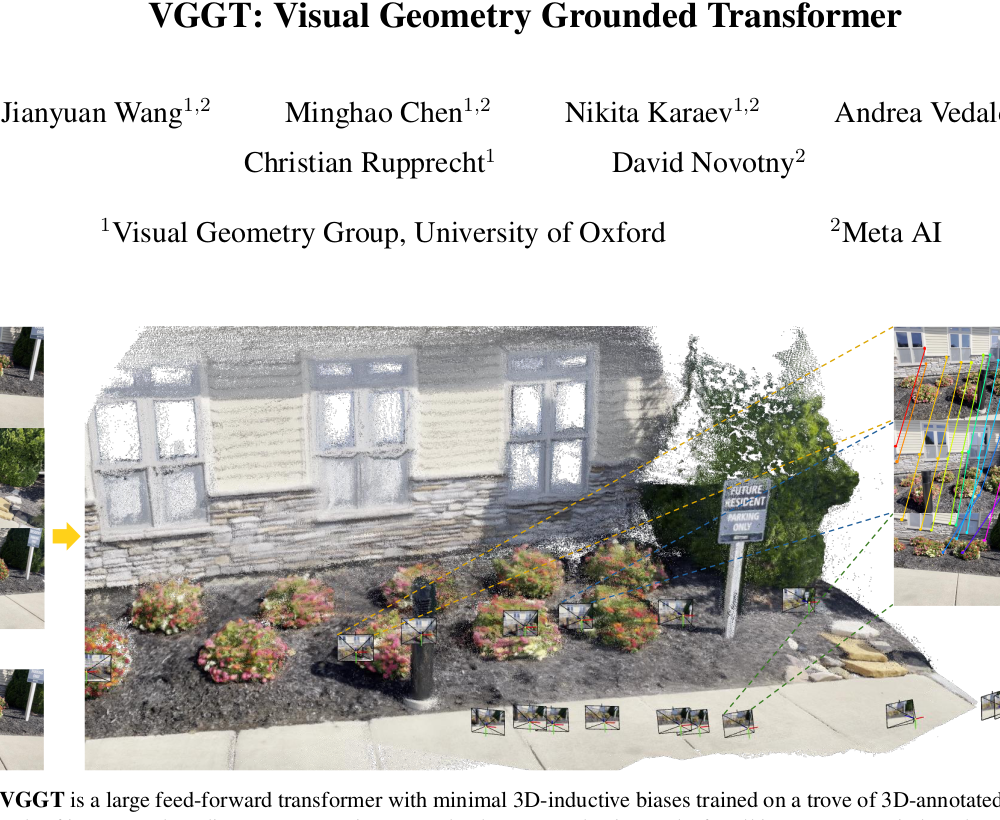
\includegraphics[width=\textwidth]{figures/vggt_fig1.png}
\caption{VGGT}
\label{fig:paper-vggt}
\end{subfigure}
\caption{DUSt3R 与 VGGT 方法图对照。来源：DUSt3R \citet{dust3r}，VGGT \citet{vggt}。}
\label{fig:paper-core}
\end{figure}

表\,\ref{tab:foundation} 进一步汇总这一分支的输入情形、主要输出、机制定位与适用条件。

\begin{table}[t]
\centering
\small
\caption{基础与多视角 3R 模型比较。}
\label{tab:foundation}
\begin{tabularx}{\textwidth}{p{2.8cm}p{2.2cm}Y Y Y}
\toprule
模型 & 输入情形 & 主要输出 & 机制定位 & 适用条件与局限 \\
\midrule
DUSt3R & \makecell[l]{图像对/\\多视角} & pointmap、confidence、派生深度与位姿 & pose-free dense pointmap regression & 范式起点，常与对齐、SfM/MVS 接口配合使用 \\
MASt3R & \makecell[l]{图像对/\\集合} & 3D-grounded correspondences & 在几何 grounding 上增强匹配 & 重点在匹配与 SfM 接口 \\
MASt3R-SfM & \makecell[l]{无约束\\图像集合} & SfM 对齐结果 & 将 MASt3R 接入传统全局流程 & 桥接匹配增强与经典全局重建 \\
Fast3R & 多图集合 & 多视角几何 & many-view one-forward-pass & 论文表格报告 1000+ 视角扩展；需保留单 A100 与分辨率条件 \\
MV-DUSt3R+ & 稀疏视角 & pointmap、NVS/Gaussian 相关输出 & 多视角 decoder 与参考视角融合 & 论文报告 12/20 视角秒级示例；官方仓库含 demo/权重 \\
VGGT & \makecell[l]{多视角\\视觉输入} & camera、depth、pointmap、tracks & 统一 visual geometry prediction & 论文和仓库均公开，适合作为多任务几何预测的通用基线 \\
\makecell[l]{MapAnything\\Pow3R} & \makecell[l]{多种\\可选条件} & metric geometry、深度、相机等 & 引入 metric/scene/camera priors & 先验提高约束，也引入条件依赖与冲突风险 \\
\bottomrule
\end{tabularx}
\end{table}

\section{视频、动态场景与 4D 重建}

许多三维重建流程默认场景在观测期间保持静态。视频输入中若存在移动物体、非刚体形变或快速相机运动，单一静态点图可能把时间变化错误地并入几何结构。Align3R 从动态视频的单目深度对齐入手，说明 Depth Anything 这类深度先验可以为跨帧一致性提供约束；但完整多视角重建仍需同时处理相机、尺度和跨帧几何的一致性\citep{align3r,depth_anything_v2}。

MonST3R 在 DUSt3R 风格的点图上进行动态场景适配，为存在运动时的逐帧几何估计提供 dynamic confidence 与 mask\citep{monst3r}。POMATO 将 pointmap matching 与 temporal motion 结合，关注动态场景中三维对应的稳定性；D\textsuperscript{2}USt3R 则将动态场景表示为 4D pointmap，并区分静态与动态像素的几何回归\citep{pomato,d2ust3r}。Easi3R 通过推理时注意力调整从既有 DUSt3R 表征中分离运动，可作为 training-free 动态修正机制的例子\citep{easi3r}。RayMap3R 利用 inference-time RayMap 与图像分支的对比识别动态干扰，其项目页将 RayMap-only 分支的静态偏置作为动态区域识别信号，并提供代码入口\citep{raymap3r}。这里需要区分两类概念：4D pointmap 和 dynamic mask 属于几何中间量，4DGS 则是可渲染表示。

\begin{table}[t]
\centering
\small
\caption{动态 3R 方法的机制对照。}
\label{tab:dynamic}
\begin{tabularx}{\textwidth}{p{2.5cm}Y Y Y}
\toprule
方法 & 动态问题入口 & 输出或中间量 & 适用条件与局限 \\
\midrule
Align3R & 动态视频中的单目深度跨帧对齐 & aligned depth、相机相关估计 & 适合作为深度先验与 3R 的桥接方法 \\
MonST3R & 运动物体破坏静态点图 & per-frame geometry、dynamic confidence/mask & 侧重动态几何与动静分离 \\
POMATO & pointmap matching 与 temporal motion 结合 & 动态重建相关点图/运动线索 & 机制应与 MonST3R、D\textsuperscript{2}USt3R 区分 \\
D\textsuperscript{2}USt3R & 动态场景的 4D pointmap & time-aware pointmap & 关注时间维度上的几何中间量 \\
Easi3R & 从既有 DUSt3R 注意力中分离运动 & training-free dynamic correction & 适合作为推理时动态修正机制 \\
RayMap3R & 利用 RayMap 的静态偏置识别动态区域 & ray/image dual-branch signal & 项目页有论文与代码入口 \\
\bottomrule
\end{tabularx}
\end{table}

\section{长序列重建中的状态、记忆与缓存}

长序列输入要求模型在有限算力下保留足够的历史几何上下文，同时避免早期错误在后续帧中持续传播。CUT3R 采用 persistent recurrent state，将连续 3D perception 组织为带状态的模型，并在输入流上递推更新\citep{cut3r}；Spann3R 引入外部 spatial memory，用于全局 pointmap 重建\citep{spann3r}。二者都处理历史信息，但前者更接近压缩状态，后者更接近可寻址的空间存储。图\,\ref{fig:paper-dynamic-stream} 并置 MonST3R 与 CUT3R 的方法图，用于对照动态几何估计和连续输入下的状态更新。

\begin{figure}[p]
\centering
\begin{subfigure}{0.96\textwidth}
\centering
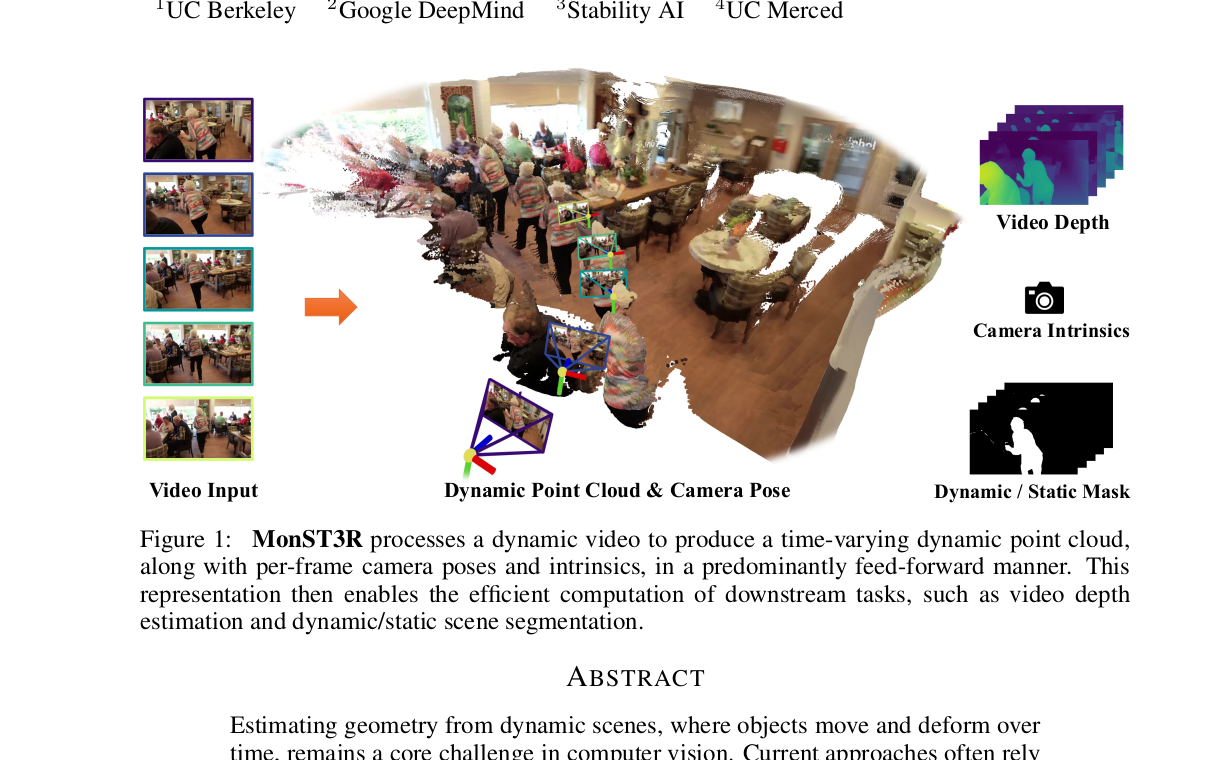
\includegraphics[width=\textwidth]{figures/monst3r_fig1.png}
\caption{MonST3R}
\label{fig:paper-monst3r}
\end{subfigure}
\vspace{0.8em}
\begin{subfigure}{0.96\textwidth}
\centering
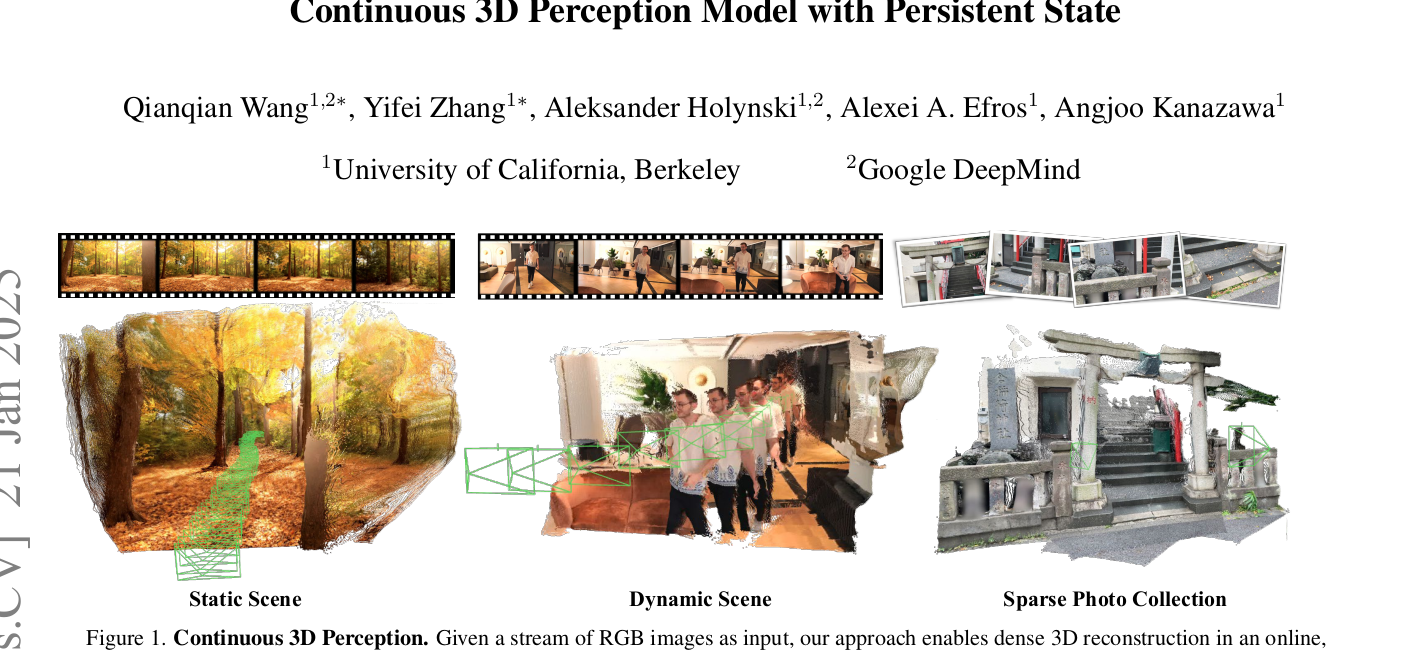
\includegraphics[width=\textwidth]{figures/cut3r_fig1.png}
\caption{CUT3R}
\label{fig:paper-cut3r}
\end{subfigure}
\caption{MonST3R 与 CUT3R 方法图对照。来源：MonST3R \citet{monst3r}，CUT3R \citet{cut3r}。}
\label{fig:paper-dynamic-stream}
\end{figure}
\FloatBarrier

近期长序列 3R 方法可以按状态组织方式进一步区分。Point3R 延续显式空间记忆方向，在 Spann3R 的基础上引入与三维场景结构相关的指针记忆，用于流式稠密重建\citep{point3r}。STream3R 在 causal transformer 框架下处理逐帧重建\citep{stream3r}，LongStream 则通过 gauge-decoupled 的关键帧位姿与正交尺度学习处理长在线序列\citep{longstream}。LONG3R 使用 memory gating 与 dual-source decoder 维持长序列上下文\citep{long3r}，LoGeR 在 parametric TTT memory 上叠加滑动窗口注意力\citep{loger}，Mem3R 将 tracking 与 mapping 的记忆显式解耦\citep{mem3r}。另一组方法关注固定预算下的信息保留：OVGGT 采用自选择缓存和动态锚点保护\citep{ovggt}，PAS3R 按位姿变化与图像频域线索调整状态更新\citep{pas3r}，FILT3R 在递推状态之上加入免训练的 Kalman 式潜变量滤波\citep{filt3r}。从公开资料看，LoGeR、Mem3R、RayMap3R 与 OVGGT 已经给出项目或代码入口，LongStream 有项目页，FILT3R 标明代码将发布，PAS3R 目前主要依据 arXiv 论文页引用；本文据此区分机制和公开状态，不进一步推断工程成熟度。

\begin{figure}[t]
\centering
\begin{tikzpicture}[
  block/.style={draw, rounded corners=2pt, fill=gray!4, minimum height=0.9cm, align=center, font=\small},
  group/.style={draw, rounded corners=2pt, fill=blue!3, minimum height=0.95cm, text width=3.6cm, align=center, font=\small},
  widegroup/.style={draw, rounded corners=2pt, fill=blue!3, minimum height=1.05cm, text width=4.25cm, align=center, font=\small},
  policy/.style={draw, rounded corners=2pt, fill=blue!3, minimum height=1.0cm, text width=4.15cm, align=center, font=\small},
  arrow/.style={-{Stealth[length=2mm]}, line width=0.45pt}
]
\node[block, minimum width=2.25cm] (input) at (0,0) {视频/图像流};
\node[group] (state) at (3.8,1.55) {递推状态\\CUT3R, STream3R};
\node[group] (spatial) at (3.8,0) {空间/指针记忆\\Spann3R, Point3R};
\node[widegroup] (hybrid) at (3.8,-1.6) {混合记忆\\LONG3R, LoGeR\\Mem3R};
\node[policy] (policy) at (8.7,0) {缓存与更新规则\\OVGGT, PAS3R\\FILT3R, LongStream};
\node[block, minimum width=2.55cm] (out) at (13.0,0) {一致点图\\深度/相机};
\draw[arrow] (input.east) -- (state.west);
\draw[arrow] (input.east) -- (spatial.west);
\draw[arrow] (input.east) -- (hybrid.west);
\draw[arrow] (state.east) -- ++(0.55,0) |- (policy.west);
\draw[arrow] (spatial.east) -- (policy.west);
\draw[arrow] (hybrid.east) -- ++(0.55,0) |- (policy.west);
\draw[arrow] (policy.east) -- (out.west);
\end{tikzpicture}
\caption{长序列 3R 中的状态和记忆机制。递推状态、空间记忆、混合记忆和缓存策略分别对应不同的更新规则。}
\label{fig:memory}
\end{figure}

\begin{table}[t]
\centering
\small
\caption{长序列与流式 3R 的记忆原语。}
\label{tab:memory}
\begin{tabularx}{\textwidth}{p{2.8cm}Y Y Y}
\toprule
类别 & 代表工作 & 主要作用 & 适用条件与局限 \\
\midrule
递推状态 & CUT3R, STream3R & 在连续输入间压缩历史几何上下文 & 早期错误可能进入后续状态；状态可解释性有限 \\
空间/指针记忆 & Spann3R, Point3R & 保存或索引与空间位置相关的重建信息 & 需要处理遮挡、重复纹理和空间漂移 \\
混合记忆 & LONG3R, LoGeR, Mem3R & 同时维护局部窗口和全局场景线索 & 内存预算、更新策略和遗忘机制影响稳定性 \\
缓存治理与滤波 & OVGGT, PAS3R, FILT3R, LongStream & 在固定预算下选择保留、更新或过滤状态 & 策略错误会造成关键信息丢失或动态物体残留 \\
\bottomrule
\end{tabularx}
\end{table}

\section{测试时验证、修正与先验输入}

3R 模型通常同时输出 pointmap、depth、camera、tracks、confidence 等几何量，这些量之间存在可检验的一致性关系。测试时机制便利用这一点，在推理阶段检查或修正跨视角、跨时间和跨输出的冲突。Test3R 使用 image triplet 之间的几何一致性进行测试时优化，将推理过程组织为轻量的 consistency adjustment\citep{test3r}；TTT3R 则把递推 3R 模型的状态更新表述为在线 test-time training，并按对齐置信度推导记忆更新速率\citep{ttt3r}。二者都利用测试时信息，但一个主要修正输出一致性，另一个主要更新内部状态。

G-CUT3R 在 CUT3R 上加入模态特异的先验编码器，使深度、相机或位姿等先验能够在推理阶段进入重建过程，可视为 prior-guided 的测试时增强\citep{gcut3r}。Pow3R 的设置不同，它把先验作为可选输入直接纳入前馈模型训练和推理\citep{pow3r}。MASt3R-SfM 则通过经典 SfM 的一致性循环对 MASt3R 匹配结果进行校验和约束，使神经匹配重新进入 bundle adjustment 等传统流程\citep{mast3r_sfm}。这些方法的差异主要在于先验或一致性约束进入系统的位置。

除模型自带的先验通道之外，3R 系统也常借用外部先验。Depth Pro、Metric3D v2 提供 metric depth 与表面法线线索，DINOv2/DINOv3 提供视觉特征，CoTracker、SpatialTracker、SAM2 给出轨迹或分割信号\citep{depth_pro,metric3dv2,dinov2,dinov3,cotracker,spatialtracker,sam2}。这些先验可补充尺度、匹配、动态识别和失败检测信息，但它们同样具有域偏置和失效区间。当外部先验与 3R 模型预测冲突时，需要额外的一致性检查或置信度策略，而不能默认先验总是正确。

\begin{table}[t]
\centering
\small
\caption{测试时机制与先验输入的进入位置。}
\label{tab:testtime}
\begin{tabularx}{\textwidth}{p{3.1cm}p{3.0cm}Y Y}
\toprule
方法或先验 & 进入位置 & 修正/约束信号 & 适用条件与局限 \\
\midrule
Test3R & \makecell[l]{测试时\\一致性优化} & image triplet 的几何一致性最大化 & 更接近一致性学习；计算开销随输入数量增长 \\
TTT3R & 在线测试时训练 & 递推状态按对齐置信度更新 & 论文和项目页报告 20 FPS / 6 GB；仍需按硬件与序列设置引用 \\
G-CUT3R & \makecell[l]{推理时\\prior guidance} & 深度/相机/位姿先验进入 CUT3R 解码 & 先验缺失或冲突时的回退行为需要在系统层处理 \\
Pow3R & 训练时条件输入 & 内参/位姿/深度等可选模态 & 先验可用性与正确性需要单独说明 \\
MASt3R-SfM & SfM 阶段后处理 & 经典 BA 与检索一致性回路 & 全局 SfM 校验路线 \\
\makecell[l]{Depth Anything /\\Depth Pro /\\Metric3D v2} & \makecell[l]{外部深度/\\法线先验} & metric/relative depth、surface normal & 零样本迁移仍受目标域分布影响，需对照失败样本 \\
\makecell[l]{DINOv2 /\\DINOv3} & \makecell[l]{视觉特征\\backbone} & 通用表征用于匹配与对齐 & 适合提供特征先验，几何一致性仍需联合校验 \\
\makecell[l]{CoTracker /\\SpatialTracker /\\SAM2} & 跟踪/分割辅助 & 长程跟踪、3D 像素跟踪、视频分割 & 分割/跟踪错误会污染动态/几何下游；适合作为辅助信号 \\
\bottomrule
\end{tabularx}
\end{table}

\section{从几何预测到可查看输出}

实际系统通常不直接消费模型内部的 pointmap，而是需要深度图、点云、mesh、相机轨迹、置信度热力图、Gaussian 表示或失败样本报告等可查看、可比较、可归档的结果。3D Gaussian Splatting 提供实时可渲染的辐射场表示，4DGS 与 4D-Rotor Gaussian Splatting 将其扩展到动态场景\citep{gaussian_splatting_3d,gaussian_splatting_4d,rotor_4dgs}。在本文语境中，Gaussian 主要是输出和渲染层；pose-free 几何估计仍由上游 3R 模型承担。

3R 与 Gaussian 表示之间已经出现若干过渡方法。Splatt3R 在 MASt3R 风格的几何上预测高斯属性，将未标定图像对映射到 Gaussian 表示\citep{splatt3r}；InstantSplat 借助稠密立体先验与 Gaussian Bundle Adjustment 处理稀疏视角\citep{instantsplat}；NoPoSplat 则从稀疏无位姿图像预测规范坐标下的高斯\citep{noposplat}。这些方法使 3R 输出更容易转为可渲染资产。应用时仍需同时检查新视角渲染、几何一致性、视角外泛化，以及代码、权重、许可证和显存条件。

\section{应用证据、复现与失败样本记录}

评估 3R 方法的应用可行性时，需要区分几类不同证据。论文中的方法图、章节说明和实验表支撑方法机制及基准结果；官方仓库提供代码、权重和 demo 状态；本地复现记录只能说明依赖、默认输入和接口是否成立；跨场景评测、失败样本和许可证条款才更接近实际使用条件。本文对归类不稳或来源尚未核对的事项保留为``尚需确认''。论文原图只在复用许可明确时嵌入，并在 caption 中保留来源。

较完整的复现记录至少应包括输入来源与规模、模型和权重版本、运行环境、主要输出、失败样本，以及许可证、耗时和显存。这样记录不是形式要求，而是为了在结果不可复现或质量判断存在争议时，能够回到具体条件进行核对。

表\,\ref{tab:application} 将这一要求落实到输出层面。模型给出预测之后，还需要记录一致性、置信度、跨视角对照和许可证信息。仅有运行成功的日志，并不足以支撑几何质量或应用可行性的结论。

\begin{table}[t]
\centering
\small
\caption{按输出层组织的应用证据清单。}
\label{tab:application}
\begin{tabularx}{\textwidth}{p{3.1cm}Y Y Y}
\toprule
输出层 & 代表方法或先验 & 质量信号 & 适用条件与局限 \\
\midrule
\makecell[l]{Depth/pointmap/\\confidence} & DUSt3R, VGGT, MV-DUSt3R+ & 尺度一致性、跨视角重投影、置信度与失败区域 & 深度图可视化需配合几何一致性检查 \\
\makecell[l]{Camera/\\tracks} & VGGT, MASt3R-SfM, CoTracker & 轨迹连续性、位姿闭环、匹配内点比例 & 轨迹输出适合与 SfM/BA 结果交叉核对 \\
\makecell[l]{Dynamic masks/\\motion} & MonST3R, Easi3R, RayMap3R, SAM2 & 动静分离、遮挡处理、跨帧稳定性 & 动态检测结果需结合时间稳定性观察 \\
\makecell[l]{Gaussian/\\4DGS} & Splatt3R, InstantSplat, NoPoSplat, 3DGS/4DGS & 新视角渲染、几何一致性、视角外泛化 & 渲染 demo 之后仍要看几何和工程条件 \\
系统报告 & 运行记录、论文表格、官方仓库 & 版本、输入、失败样本、许可证、显存与耗时 & 接口成立只是质量评估的起点 \\
\bottomrule
\end{tabularx}
\end{table}

\section{开放问题与结论}

近期 3R 文献中反复出现几类失败模式。弱纹理与纯色区域容易导致 pointmap 置信度下降，大片墙面或地面上的几何也更容易漂移。镜面、玻璃和强反射表面会引入反射几何，与真实几何不一致，室内场景中尤其常见。MonST3R、POMATO 等动态方法通过 dynamic mask 或 motion modeling 缓解运动干扰，但在大幅运动、频繁遮挡或非刚体变化较强的视频中仍会退化。长基线和大视差是另一类边界条件，成对预测在视差超出训练分布时一致性下降，需要匹配增强或 SfM 校验补充约束。流式与长序列方法在数百帧之后可能累积尺度和位姿误差，记忆策略与 gauge 处理会影响误差增长。域外场景同样需要谨慎，例如水下、遥感、医学或显微图像通常不在主要训练分布内，可靠判断应依赖专门评测。

从研究线索看，DUSt3R 之后的 3R 文献面临几组尚未完全解决的张力。VGGT、MapAnything 等统一模型试图同时输出多种几何量，但不同输入条件下的可靠性并不相同，因此“支持某种输入”不能直接等同于“该输入下结果可靠”。动态建模和长序列记忆都涉及时间信息，但前者关心场景或物体本身的变化，后者关心历史上下文如何保存、更新和遗忘。Test3R、TTT3R、G-CUT3R 等测试时机制提高了适配能力，也引入额外计算开销、收敛条件和先验冲突。Gaussian 输出使可视化更直接，但重投影误差、跨视角一致性、视角外表现和许可证约束仍需单独检查。

总体来看，DUSt3R 之后的 3R 谱系已经超出单纯点图预测的范围。中间表示如何选择，状态如何在长序列中维护，外部先验在哪一步进入，最后由何种表示承担可视化和资产输出，都会影响方法在实际场景中的适用性。现阶段的综述和复现工作不应只记录 benchmark 数字，也需要记录失败样本、输入条件和许可证等更接近应用边界的因素。

\bibliographystyle{unsrtnat}
\bibliography{references}

\end{document}
